% ****** Start of file apssamp.tex ******
%
%   This file is part of the APS files in the REVTeX 4.1 distribution.
%   Version 4.1r of REVTeX, August 2010
%
%   Copyright (c) 2009, 2010 The American Physical Society.
%
%   See the REVTeX 4 README file for restrictions and more information.
%
% TeX'ing this file requires that you have AMS-LaTeX 2.0 installed
% as well as the rest of the prerequisites for REVTeX 4.1
%
% See the REVTeX 4 README file
% It also requires running BibTeX. The commands are as follows:
%
%  1)  latex apssamp.tex
%  2)  bibtex apssamp
%  3)  latex apssamp.tex
%  4)  latex apssamp.tex
%
\documentclass[%
 preprint,
%superscriptaddress,
%groupedaddress,
%unsortedaddress,
%runinaddress,
%frontmatterverbose, 
%preprint,
%showpacs,preprintnumbers,
%nofootinbib,
%nobibnotes,
%bibnotes,
 amsmath,amssymb,
 aps,
%pra,
%prb,
%rmp,
%prstab,
%prstper,
%floatfix,
]{revtex4-1}

\usepackage{graphicx}% Include figure files
\usepackage{dcolumn}% Align table columns on decimal point
\usepackage{bm}% bold math
\usepackage{hyperref}% add hypertext capabilities
%\usepackage[mathlines]{lineno}% Enable numbering of text and display math
%\linenumbers\relax % Commence numbering lines

%\usepackage[showframe,%Uncomment any one of the following lines to test 
%%scale=0.7, marginratio={1:1, 2:3}, ignoreall,% default settings
%%text={7in,10in},centering,
%%margin=1.5in,
%%total={6.5in,8.75in}, top=1.2in, left=0.9in, includefoot,
%%height=10in,a5paper,hmargin={3cm,0.8in},
%]{geometry}

\usepackage{braket} % Allows for Dirac notation
\usepackage{subcaption}

\newcommand{\veff}{\hat{V}_{12,\text{eff}}}
\newcommand{\rhozero}{\rho_{\text{I}=0}}
\newcommand{\rhoone}{\rho_{\text{I}=1}}

\newcommand{\yukawa}[1]{\frac{e^{-m_\pi |#1|}}{4\pi |#1|}}
\newcommand{\yukawadimless}[1]{\frac{e^{-m_\pi #1}}{m_\pi #1}}
\newcommand{\yukawanoabs}[1]{\frac{e^{-m_\pi #1}}{4\pi #1}}

\newcommand{\rot}{\vec{r}_{12}}
\newcommand{\rotp}{\vec{r}_{12}\!\!'}

\newcommand{\taudot}{\vec{\tau}_1\cdot\vec{\tau}_2}
\newcommand{\sigmadot}{\vec{\sigma}_1\cdot\vec{\sigma}_2}

\newcommand{\lvec}[1]{\reflectbox{\ensuremath{\vec{\reflectbox{\ensuremath{#1}}}}}}

\newcommand{\threej}[6]{ \begin{pmatrix}
  #1 & #2 & #3 \\
  #4 & #5 & #6 
 \end{pmatrix}}

\newcommand{\sixj}[6]{ \begin{Bmatrix}
  #1 & #2 & #3 \\
  #4 & #5 & #6 
 \end{Bmatrix}}

\newcommand{\ninej}[9]{ \begin{Bmatrix}
  #1 & #2 & #3 \\
  #4 & #5 & #6 \\
  #7 & #8 & #9
 \end{Bmatrix}}

\begin{document}

\preprint{APS/123-QED}

\title{Energy spectra of two interacting fermions with spin-orbit coupling in a harmonic trap}% Force line breaks with \\
%\thanks{A footnote to the article title}%

\author{Cory D. Schillaci}
\affiliation{%
Department of Physics, University of California, Berkeley, California 94720, USA
}%

\author{Thomas C. Luu}%
\email{
t.luu@fz-juelich.de
}
\affiliation{
Institute for Advanced Simulation, Forschungszentrum J\"{u}lich, D�52425 J\"{u}lich, Germany
}
\affiliation{Institut f\"{u}r Kernphysik and J\"{u}lich Center for Hadron Physics,
Forschungszentrum J\"{u}lich, D�52425 J\"{u}lich, Germany}%Lines break automatically or can be forced with \\

\date{\today}% It is always \today, today,
             %  but any date may be explicitly specified

\begin{abstract}
We explore the two body spectra of spin-$1/2$ fermions in isotropic harmonic traps with external spin-orbit potentials and short range two body interactions. Nonperturbative results are presented for pure Rashba, equal parts Rashba and Dresselhaus, and Weyl type spin-orbit couplings. 
%Matrix elements are calculated in a basis of total angular momentum eigenstates to best expose the underlying symmetries 
\end{abstract}

%\pacs{Valid PACS appear here}% PACS, the Physics and Astronomy
                             % Classification Scheme.
%\keywords{Suggested keywords}%Use showkeys class option if keyword
                              %display desired
\maketitle

%\tableofcontents

\section{\label{sec:level1}Introduction}

Cold atomic gases with spin-orbit coupling (SOC) have recently been an area of intense interest because of the potential to create exotic condensed matter systems with precisely tunable interactions\cite{nature11841}. SOC was first realized in a Bose condensate of $^{87}$Rb \cite{nature09887} and extended shortly after to Fermi gases of $^{40}$K\cite{PhysRevLett.109.095301} and $^6$Li\cite{PhysRevLett.109.095302}. These spin-orbit interactions are `synthetic' in the sense that hyperfine states stand in as virtual spin states. 


\section{Spin Orbit interactions}
In this paper we consider three different types of spin-orbit coupling (SOC). The form of spin-orbit coupling realized in experiments is a linear combination of the Rashba\cite{0022-3719-17-33-015} and Dresselhaus\cite{PhysRev.100.580} types,
\begin{align}
V_{R}&=\alpha_R (\sigma_x k_y-\sigma_y k_x) \label{eq:Rashba},\\
V_{D}&=\alpha_D (\sigma_x k_y+\sigma_y k_x) \label{eq:Dresselhaus},
\end{align} 
which were originally recognized in two-dimensional solid state systems. In a two-dimensional system, these form a complete basis for spin-orbit couplings linear in momentum. Note that some references use the alternate definitions $V_R\propto  (\sigma_x k_x+\sigma_y k_y) $ and $V_D\propto  (\sigma_x k_x-\sigma_y k_y) $ which are equivalent up to a pseudospin rotation. The simplest scenario for which the Rashba SOC arises is the case of electrons in the presence of a static electric field. Electrons moving with respect to the lab frame will experience a magnetic field due to Lorentz invariance, which leads to a velocity dependent Zeeman effect of the form \eqref{eq:Rashba}. Dresselhaus type interactions ???

To date, experiments have only produced SOC potentials in which the Rashba and Dresselhaus terms appear with equal strength. This unidirectionally couples the pseudo-spin and momentum along a single axis,
\begin{equation}
\label{eq:R=D}
V_{R=D}=\alpha_{R=D}\sigma_x k_y,
\end{equation} 
however a proposal for tuning the ratio $\alpha_R/\alpha_D$ has been given in \cite{PhysRevA.84.025602}.  An experimental setup which gives the simple three-dimensional Weyl coupling,
\begin{equation}\label{eq:Weyl}
V_{W}=\alpha_W \vec{k}\cdot\vec{\sigma},
\end{equation}
has also been proposed in \cite{PhysRevLett.108.235301} and \cite{PhysRevLett.111.125301}. The single particle energy levels for this coupling were found numerically in \cite{0953-4075-46-13-134003}.

In this paper we calculate the spectra of two particles with a short-range two-body interaction, an isotropic harmonic trapping potential and spin-orbit coupling. The single particle Hamiltonian is,
\begin{equation}
H_1=\frac{\hbar^2 k^2}{2m}+\frac{1}{2}m\omega^2 r^2 + V_{SO}.
\end{equation}
For the spin-orbit term $V_{SO}$, we consider equal Rashba and Dresselhaus \eqref{eq:R=D}, pure Rashba \eqref{eq:Rashba}, and Weyl spin-orbit couplings\eqref{eq:Weyl}. 

The particles also interact via a short-ranged s-wave interaction, 
\begin{equation}
V_2 \ket{\vec{k}_1;\vec{k}_2}=\lim_{\Lambda\rightarrow\infty}\frac{4\pi \hbar^2}{m}a(\Lambda)f(|\vec{k}_1-\vec{k}_2|/\Lambda)\ket{\vec{k}_1;\vec{k}_2}
\end{equation}
where $f(x)$ refers to some regulator and $a(\Lambda)$ is the renormalized coupling which reproduces the s-wave scattering length $a$ independent of the regulator form and regularization scale. 


\section{Weyl coupling}
We tackle the Weyl form first because of its mathematical simplicity. Our approach is to determine the matrix elements of the SOC, then make use of the known analytic spectrum of two interacting particles in a harmonic trap\cite{Busch} to find an eigenvalue equation. This equation is solved numerically at the desired precision by choosing an appropriately large truncated basis of harmonic oscillator eigenstates.

As usual, the two-body problem is best approached in the dimensionless Jacobi coordinates,
\begin{equation}
R=\frac{r_1+r_2}{\sqrt{2}b}, \qquad r=\frac{r_1-r_2}{\sqrt{2}b},
\end{equation}
and the corresponding conjugate momenta $q,Q$ representing the relative and total momenta. For an isotropic harmonic oscillator, distances can be expressed in terms of the ground state length scale $b=\sqrt{\hbar/m\omega}$ and energies will be similarly measured in units of $E_0=\hbar\omega$. We also define the spin operators
\begin{equation}
\vec{\sigma}=\vec{\sigma}_1-\vec{\sigma}_2, \qquad \vec{\Sigma}=\vec{\sigma}_1+\vec{\sigma}_2.
\end{equation}

 With these definitions, the two-body Hamiltonian can be separated into relative and center of mass parts,
\begin{equation}\label{eq:WeylHamiltonian}
\frac{1}{\hbar\omega}H=\left(h_{0,\text{rel}}+\frac{\tilde{\alpha}_W}{\sqrt{2}} \vec{q}\cdot\vec{\sigma} + \sqrt{2}\pi \tilde{a}(\Lambda) \delta^{(3)}(r)\right)+\left(h_{0,\text{CM}}+\frac{\tilde{\alpha}_W}{\sqrt{2}} \vec{Q}\cdot\vec{\Sigma} \right)
\end{equation}
Notably, the spin-orbit coupling appears in both terms. The tilde over the coupling constants indicates that they are dimensionless, related to the original coupling constants by dividing out the oscillator length (e.g. $\tilde{\alpha}=\alpha/b$).

Eigenstates of the harmonic oscillator trapping potential form a convenient basis for these calculations. There are many possible combinations of complete basis states to choose from, and we choose the particular angular momentum eigenstates,
\begin{equation}\label{eq:basisStates}
\ket{n(ls)j;NL;(jL)J},
\end{equation}
which simplify the matrix elements for the relative coordinate operators. Here $n,l$ correspond to the relative HO quantum numbers, and $N,L$ the center of mass HO quantum numbers. We use the convention that $n,N=0,1,2,\dots$, therefore $E=2n+l+2N+L+3$. The total spin of the two spin-$1/2$ particles is denoted by $s = s_1 + s_2$ and may be either 0 or 1. Total spin $s$ is first coupled with $l$ to make angular momentum $j$, which is then recoupled with the CM angular momentum $L$ to make the state's total angular momentum $J$. Because all terms in the Hamiltonian \eqref{eq:WeylHamiltonian} are scalars, the interaction is independent of $J_z$ and so we omit this quantum number for clarity. Due to Pauli exclusion, $l + s$ must be even to enforce antisymmetry under exchange of the particles.

%These basis states are eigenstates of the relative and CM parts of the HO Hamiltonian separately, i.e.
%\begin{align}
%h_{0,\text{rel}}\ket{n(ls)j;NL;(jL)J}&=(2n+l+3/2)\ket{n(ls)j;NL;(jL)J}, \\
%h_{0,\text{CM}}\ket{n(ls)j;NL;(jL)J}&=(2N+L+3/2)\ket{n(ls)j;NL;(jL)J}.
%\end{align}

Standard angular momentum algebra can be used to determine the matrix elements of the two spin-orbit coupling terms, we follow the conventions of \cite{Edmonds}. For Weyl SOC coupling of two spin-$1/2$ fermions, the matrix elements of the coupling in the relative momentum are
\begin{equation}\label{eq:WeylRel}\begin{split}
\bra{n'(l's')j';N'L';(j'L')J'}\vec{q}&\cdot\vec{\sigma} \ket{n(ls)j;NL;(jL)J} = \\
&\delta_{N,N'}\delta_{L,L'}\delta_{j,j'}\delta_{J,J'}(-1)^{l+s'+j} 
 2\sqrt{3}(s'-s)\sixj{j}{s'}{l'}{1}{l}{s} \braket{n'l' || q || n l}
\end{split}
\end{equation}
Which is nonzero only if $s\neq s'$, i.e. the operator changes the total spin of the two particles as expected for a parity violating potential. The reduced matrix element of the momentum operator is given by
\begin{align}
\braket{n'l' || q || n l}=&(-1)^{l'}(-1)^{\frac{l+l'+1}{2}}\sqrt{\frac{2(2l+1)(2l'1+1)}{(l+l'+1)}}\braket{n'l'0| (-i \nabla_0) | n l 0} \\
\begin{split} =& i(-1)^{l}\sqrt{\frac{l+l'+1}{2}}\sqrt{n!n'!\Gamma(n+l+3/2)\Gamma(n'+l'+3/2)} \\ 
&\times\sum_{m,m'=0}^{n,n'} \left\{
     \begin{array}{lr}
       \frac{(-1)^{m+m'}\left[2m\Gamma\left(m+m'+1+\frac{l+l'}{2}\right)-\Gamma\left(m+m'+1+\frac{l+l'}{2}\right)\right]}{m!m'!(n-m)!(n'-m')!\Gamma(m+l+3/2)\Gamma(m'+l'+3/2)} & \text{if}\: l'=l-1 \\
        \frac{(-1)^{m+m'+1}\left[(2m+2l+1)\Gamma\left(m+m'+1+\frac{l+l'}{2}\right)-\Gamma\left(m+m'+1+\frac{l+l'}{2}\right)\right]}{m!m'!(n-m)!(n'-m')!\Gamma(m+l+3/2)\Gamma(m'+l'+3/2)} & \text{if}\: l'=l+1 \\
       0 & \text{otherwise}
     \end{array}
   \right.
   \end{split}
\end{align}
The relative momentum coupling from the Weyl SOC operator connects states with different parity while preserving the antisymmetry of the state by also changing the total spin $s$, leaving $l+s$ even.

Our choice of basis makes this matrix element simple at the cost of complicating the center-of-mass term. We take the approach of expanding the states \eqref{eq:basisStates} in the alternate coupling scheme 
\begin{equation}\label{eq:basisStates2}
\ket{n(ls)j;NL;(jL)J}=(-1)^{l+s+L+J}\sqrt{2j+1}\sum_{\mathcal{J}}\sqrt{2\mathcal{J}+1}\sixj{l}{s}{j}{L}{J}{\mathcal{J}}\ket{nl;N(Ls)\mathcal{J};(l\mathcal{J})J}
\end{equation}
Using this notation, the matrix elements can be written
\begin{equation}\begin{split}
\bra{n'(l's')j';N'L';(j'L')J'}&\vec{Q}\cdot\vec{\Sigma} \ket{n(ls)j;NL;(jL)J} = \delta_{n,n'}\delta_{l,l'}\delta_{J,J'}\delta_{s,1}\delta_{s1,1} (-1)^{L} 2\sqrt{6} \\
&\times\braket{N'L'|| \vec{Q} || NL} \sum_{\mathcal{J}}(-1)^\mathcal{J} (2\mathcal{J}+1)\sixj{l}{1}{j'}{L'}{J}{\mathcal{J}}\sixj{l}{1}{j}{L}{J}{\mathcal{J}}\sixj{\mathcal{J}}{1}{L'}{1}{L}{1}.
\end{split}
\end{equation}
This time, the reduced matrix element of the CM momentum changes the parity by connecting states with $\Delta L=1$. Matrix elements are non-zero only for $\Delta s=0$ because the antisymmetry of the wave function depends only on $l$ which does not change. We also note that the CM term does not affect states with singlet spin wave functions ($s=0$).

For the remaining part of the Hamiltonian, we can rewrite the Schr\"{o}dinger equation in an integral form 
\begin{equation}\label{eq:integralForm}
\frac{1}{\epsilon - H_{0,rel}- H_{0,CM}-\sqrt{2}\pi \tilde{a}(\Lambda)\delta^{(3)}(r)}\frac{\tilde{\alpha}_W}{\sqrt{2}}\left(\vec{q}\cdot\vec{\sigma}+\vec{Q}\cdot\vec{\Sigma}\right) \ket{\psi}=\ket{\psi}.
\end{equation}
The advantage of the form \eqref{eq:integralForm} is that the spectrum of the Hamiltonian without SOC has been determined exactly in \cite{Busch}. The Green's function can be found by writing
\begin{equation}
\frac{1}{\epsilon - H_{0,rel}- H_{0,CM}-\sqrt{2}\pi \tilde{a}(\Lambda)\delta^{(3)}(r)}=G_0(\epsilon)+G_0(\epsilon)T(\epsilon)G_0(\epsilon)
\end{equation}
and determining the $T$-matrix elements from the infinite sum,
\begin{equation}
T(\epsilon)=\tilde{V}_2+G_0(\epsilon)\tilde{V}_2G_0(\epsilon)+\dots=\delta_{N,N'}\delta_{L,L'}\delta{s,0}\delta_{s',0}\delta_{l,0}\delta_{l',0}\delta_{j,j'}\delta_{J,J'}\frac{\sqrt{2}\pi\sqrt{\frac{\Gamma(n+3/2)\Gamma(n'+3/2)}{n!n'!}}}{\frac{1}{\tilde{a}}-\sqrt{2}\frac{\Gamma\left(\frac{3}{4}-\frac{\epsilon-2N-L-3/2}{2}\right)}{\Gamma\left(\frac{1}{4}-\frac{\epsilon-2N-L-3/2}{2}\right)}}
\end{equation}

\begin{figure}
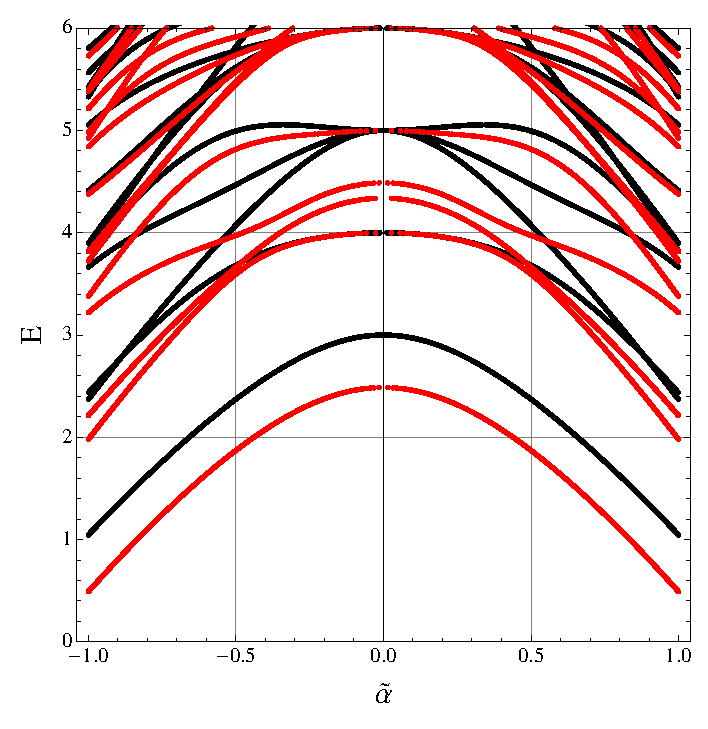
\includegraphics[width=0.5\linewidth]{Figures/WeylMinusOne}\nobreak
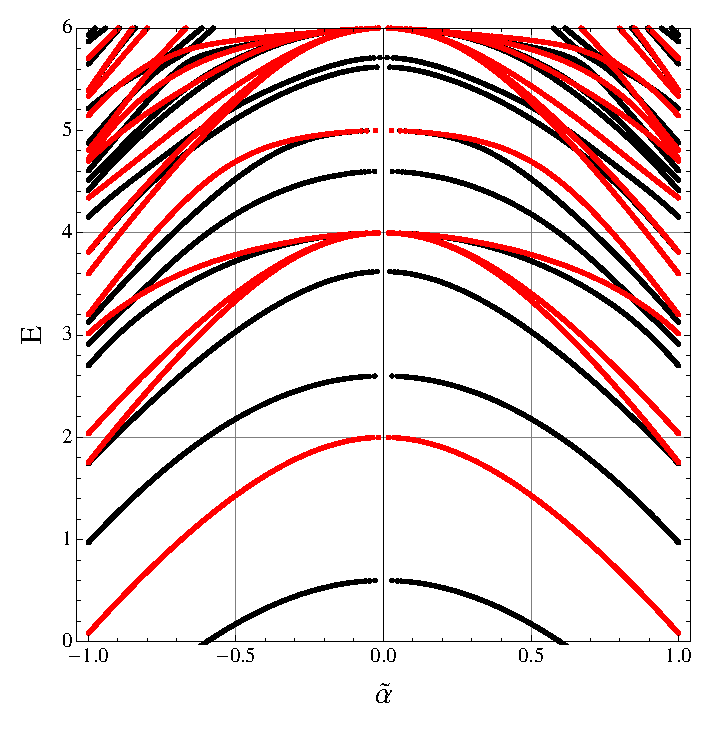
\includegraphics[width=0.5\linewidth]{Figures/WeylPOneInfinity}
\caption{\label{fig:WeylSpectrum} Spectrum of states with total angular momentum $J=0$ for the Hamiltonian \eqref{eq:WeylHamiltonian}. The left figure shows the energies without the two-body interaction, i.e. $\tilde{a}=0$ (black), and with negative scattering length $\tilde{a}=-1$ (red). The right figure shows the results for a positive scattering scattering length $\tilde{a}=1$ (black) and in the unitary limit $\tilde{a}\rightarrow\infty$ (red).} 
\end{figure}

Using this approach, we calculated the spectrum of the two interacting particles with Weyl spin-orbit coupling. To calculate the spectrum, one determines the values of the two-body energy $E=\epsilon\,\hbar\omega$ for which the operator on the left hand side has an eigenvalue of $1$. Note that, given a particular choice of $\epsilon$ and $\tilde{a}$, determining values of $\alpha$ for which a solution to \eqref{eq:integralForm} exists is particularly simple. Our calculations are performed in a truncated basis of the harmonic oscillator states \eqref{eq:basisStates}, where a cutoff $2N+L+2n+l\leq N_{max}$ is set high enough that the eigenvalues of the matrix have converged to the desired accuracy.  For $N_\text{max}=?$ we find convergence to ? decimal places. The energy spectrum is shown in Figure \ref{fig:WeylSpectrum}.

\section{The Pure Rashba SOC}

In order to find the matrix elements of the pure Rashba coupling given in \eqref{eq:Rashba}, we first note that it can be written as a spherical tensor,
\begin{equation}
V_{R}=i\sqrt{2}\:\alpha_R \left[ k \otimes \sigma \right]_{10}.
\end{equation}
We therefore have the two-body Hamiltonian,
\begin{equation}\label{eq:RashbaHamiltonian}
\frac{1}{\hbar\omega}H=\left(h_{0,\text{rel}}+i \tilde{\alpha}_R  \left[ \vec{q} \otimes \vec{\sigma} \right]_{10} + \sqrt{2}\pi \tilde{a}(\Lambda) \delta^{(3)}(r)\right)+\left(h_{0,\text{CM}}+i \tilde{\alpha}_R [ \vec{Q}\otimes \vec{\Sigma} ]_{10} \right).
\end{equation}

Because the spin orbit coupling is now a $k=1$ tensor rather than a scalar operator, the angular momentum couplings do not simplify as much as before. Additionally, we must now track the magnetic quantum number $J_z$ because the matrix elements now depend on it. For the relative coordinate part of the SOC, some algebra gives
\begin{equation}\begin{split}
&\bra{n'(l's')j';N'L';(j'L')J'J'_z}  [ \vec{q} \otimes \vec{\sigma} ]_{10}  \ket{n(ls)j;NL;(jL)JJ_z} =6 (-1)^{J+J'-J'_z+j'+L+1}\delta_{N,N'}\delta_{L,L'}\delta_{J_z,J'_z} \\
 &\times\sqrt{(2J+1)(2J'+1)(2j+1)(2j'+1)} \threej{J'}{1}{J}{-J_z}{0}{J_z} \sixj{j'}{J'}{L}{J}{j}{1}
 \renewcommand{\arraystretch}{0.9}
 \ninej{\hphantom{l}l'\hphantom{l}}{\hphantom{l}l\hphantom{l}}{\hphantom{l}1\hphantom{l}}{s'}{s}{1}{j'}{j}{1} (s'-s) \braket{n'l' || q || n l},
\end{split}
\end{equation}
This expression presents somewhat more numerically difficulty than \eqref{eq:WeylRel} because of the dependence on many Wigner $j$ symbols.

For the CM part of the Hamiltonian we again expand the basis states in the alternate coupling scheme to obtain the matrix elements,
\begin{equation}\begin{split}
&\bra{n'(l's')j';N'L';(j'L')J'J'_z} [ \vec{Q} \otimes \vec{\Sigma} ]_{10}  \ket{n(ls)j;NL;(jL)JJ_z} = \delta_{n,n'}\delta_{l,l'}\delta_{J_z,J'_z}\delta_{s,1}\delta_{s',1} \\
 &\quad\times6\sqrt{2}(-1)^{J+J'-J'_z+l} \sqrt{(2J+1)(2J'+1)(2j+1)(2j'+1)} \threej{J'}{1}{J}{-J_z}{0}{J_z}  \braket{N' L' || Q || N L} \\ 
 &\quad\times\sum_{\mathcal{J},\mathcal{J}'} (-1)^\mathcal{J}(2\mathcal{J}+1)(2\mathcal{J}'+1)\sixj{l}{1}{j'}{L'}{J'}{\mathcal{J}'}\sixj{l}{1}{j}{L}{J}{\mathcal{J}}\sixj{\mathcal{J}'}{J'}{l}{J}{\mathcal{J}}{1}
 \renewcommand{\arraystretch}{0.9}
 \ninej{\hphantom{l}L'\hphantom{l}}{\hphantom{l}L\hphantom{l}}{\hphantom{l}1\hphantom{l}}{1}{1}{1}{\mathcal{J}'}{\mathcal{J}}{1} .
\end{split}
\end{equation}

\section{Rashba=Dresselhaus SOC}

Energy levels of the two-body system the one-dimensional equivalent of this Hamiltonian with the additional magnetic field couplings present in experimental realizations have been calculated by \cite{arXiv:1406.7177}.

\section{Conclusions}

\bibliography{References}
\end{document}
%
% ****** End of file apssamp.tex ******
